\documentclass[a4paper]{article}
\usepackage{polski}
\usepackage[utf8]{inputenc}
\usepackage{enumerate}
\usepackage{graphicx}
\usepackage{float} 
\usepackage{indentfirst}

\usepackage{geometry}
\newgeometry{tmargin=2.5cm, bmargin=2cm, lmargin=1.5cm, rmargin=2cm}

\title{Architektura oprogramowania}
\date{}
\author{}

\begin{document}
\maketitle

\section{Diagram węzłów}

\begin{figure}[H]
\centering
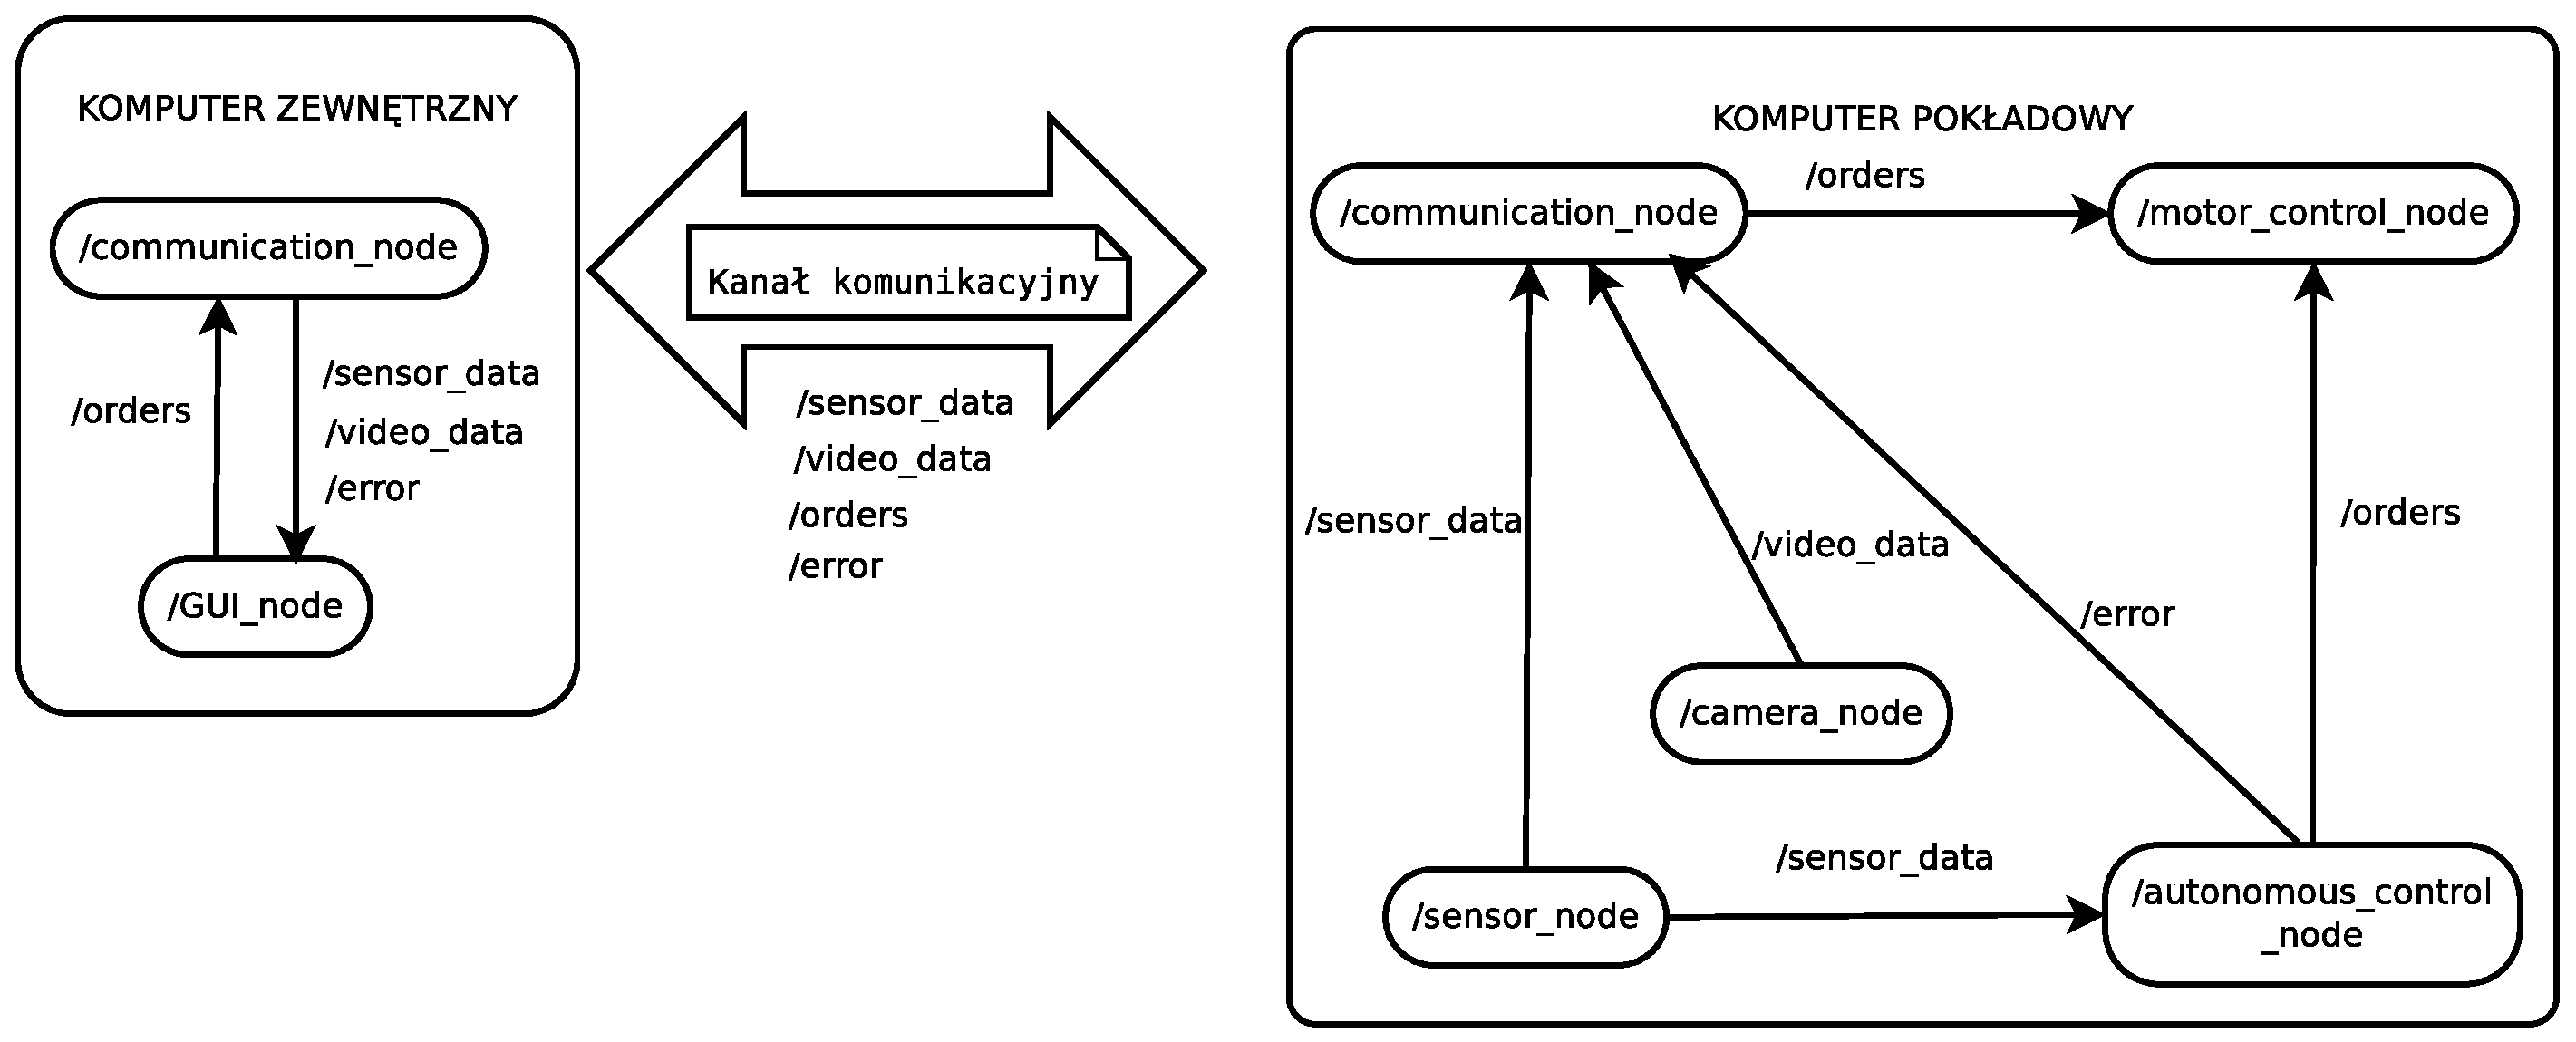
\includegraphics[width=16cm]{architektura}
\caption{Diagram komponentów programowych przedstawionych jako węzły i tematy ROSa}
\end{figure}

Powyższy rysunek jest rozwinięciem diagramu komponentów programowych (założenia projektowe, rysunek 2), uwzględniającym szczegóły implementacyjne na poziome pojedynczych węzłów i tematów ROSa. Tematy oznaczone są jako nazwy nad strzałkami łączącymi komponenty. Służą one do przekazywania między węzłami konkretnego typu danych. Typy danych opisane są szczegółowo w sekcji \ref{opis_typow}.

\section{Opis węzłów}

\begin{table}[H]
\begin{center}
\begin{tabular}[t]{ | p{3.5cm} | p{7cm} | p{3cm} | p{3cm} | } 
\multicolumn{1}{c}{Nazwa węzła} & \multicolumn{1}{c}{Opis} & 
\multicolumn{1}{c}{Subskrybowane tematy} & \multicolumn{1}{c}{Publikacje} \\
\hline \verb|/communication_node| & Zajmuje się transmisją danych pomiędzy maszynami. Analogiczny węzeł działa na komputerze zewnętrznym, przy odwrotnym stanie tematów subskrybowanych/publikacji & \verb|/sensor_data| \verb|/video_data| \verb|/error| & \verb|/orders|\\
\hline \verb|/sensor_node| & Publikuje informacje z czujników \ podłączonych do GPIO Raspberry Pi & - & \verb|/sensor_data| \\ 
\hline \verb|/camera_node| & Publikuje dane z kamery & - & \verb|/video_data|\\
\hline \verb|/autonomous_| \verb|control_node| & Podejmuje decyzje o awaryjnym zatrzymaniu robota. Gdy taka sytuacja nastąpi, przesyła odpowiednią informację użytkownikowi. & \verb|/sensor_data| & \verb|/orders| \verb|/error|\\
\hline \verb|/motor_control_node| & Na podstawie otrzymanych rozkazów generuje sygnały sterujące silnikami & \verb|/orders| & - \\
\hline \verb|/GUI_node| & Stanowi interfejs dla użytkownika. Pozwala na wydawanie rozkazów oraz podgląd obrazu z kamery i czujników & \verb|/sensor_data| \verb|/video_data| \verb|/error| & \verb|/orders| \\
\hline
\multicolumn{1}{c}{} & \multicolumn{1}{l}{} & 
\multicolumn{1}{l}{} & \multicolumn{1}{c}{} \\ 
\end{tabular}
\caption{Lista głównych komponentów programowych oraz ich danych wejściowych i wyjściowych }
\end{center}
\end{table}

\newgeometry{tmargin=2.5cm, bmargin=2cm, lmargin=3cm, rmargin=3cm}

Węzły są najbardziej intuicyjną reprezentacją komponentów programowych. Są to równolegle działające procesy wykonujące wyspecjalizowane zadania. Dzięki mechanizmowi subskrybowania i publikowania wiadomości w tematach, można w łatwy i wyraźny sposób określić ich dane wejściowe i wyjściowe. Zgodnie z dobrą praktyką programistyczną, węzły nazwane są w języku angielskim. 

\section{Opis typów danych} \label{opis_typow}

Zgodnie z mechanizmem systemu ROS, każdy temat ma przypisany swój konkretny typ danych. Poniżej znajduje się lista typów używanych w projekcie. Większość z nich to typy złożone. Zagnieżdżenie typów - zgodnie z konwencją stosowaną w ROSie - oznaczone jest poprzez wcięcia. Jako że niektóre typy danych muszą być skrojone dokładnie na miarę robota (np. dane z czujników), utworzona zostanie specjalna paczka \verb|LIGO_msgs|, w której będą one zawarte. 

\begin{itemize}

\item Temat \verb|/video_data|
\begin{verbatim}
sensor_msgs/Image video
  std_msgs/Header header
    uint32 seq
    time stamp
    string frame_id
  uint32 height
  uint32 width
  string encoding
  uint8 is_bigendian
  uint32 step
  uint8[] data
\end{verbatim}

\item Temat \verb|/sensor_data|
\begin{verbatim}
LIGO_msgs/Sensor_data data
  uint8 left_sensor
  uint8 mid_sensor
  uint8 right_sensor
  bool contactor1
  bool contactor2
  bool contactor3
  bool contactor4
  bool contactor5
  bool contactor6
  bool contactor7
  bool contactor8
\end{verbatim}

\item Temat \verb|/orders|
\begin{verbatim}
LIGO_msgs/Order_data order
  int8 left_velocity
  int8 right_velocity
  bool priority
\end{verbatim}

\item Temat \verb|/error|
\begin{verbatim}
int8 error_code
\end{verbatim}

\end{itemize}

\section{Podział obowiązków i podsumowanie}

Za wszystkie komponenty wchodzące w skład oprogramowania komputera pokładowego odpowiedzialny jest Piotr Dulewicz. Napisaniem programów działających na komputerze zewnętrznym zajmuje się Piotr Jabłoński. Komunikacją zajmuje się Andrzej Szmyt. 

Dzięki dokładnie zdefiniowanym typom danych system jest spójny, i połączenie kilku niezależnie tworzonych części oprogramowania nie powinno sprawiać problemów.


\end{document}